
%%%%%%%%%%%%%%%%%%%%%%%%%%%%%%%%%%%%%%%%%
% Programming/Coding Assignment
% LaTeX Template
%
% This template has been downloaded from:
% http://www.latextemplates.com
%
% Original author:
% Ted Pavlic (http://www.tedpavlic.com)
%
% Note:
% The \lipsum[#] commands throughout this template generate dummy text
% to fill the template out. These commands should all be removed when 
% writing assignment content.
%
% This template uses a Perl script as an example snippet of code, most other
% languages are also usable. Configure them in the "CODE INCLUSION 
% CONFIGURATION" section.
%
%%%%%%%%%%%%%%%%%%%%%%%%%%%%%%%%%%%%%%%%%

%----------------------------------------------------------------------------------------
%	PACKAGES AND OTHER DOCUMENT CONFIGURATIONS
%----------------------------------------------------------------------------------------



\documentclass{article}

\usepackage{fancyhdr} % Required for custom headers
\usepackage{lastpage} % Required to determine the last page for the footer
\usepackage{extramarks} % Required for headers and footers
\usepackage[usenames,dvipsnames]{color} % Required for custom colors
\usepackage{graphicx} % Required to insert images
\usepackage{listings} % Required for insertion of code
\usepackage{courier} % Required for the courier font
\usepackage{lipsum} % Used for inserting dummy 'Lorem ipsum' text into the template
\usepackage{setspace}
\usepackage{color}
\usepackage{comment}
\usepackage{caption}
\usepackage[T1]{fontenc}
\usepackage{hyperref}
%\usepackage{natbib}
\usepackage{underscore}
\usepackage{subfigure}
\usepackage{fixltx2e}

\hypersetup{
    colorlinks=true,
    linkcolor=blue,
    filecolor=magenta,      
    urlcolor=cyan,
    breaklinks=true
}

\usepackage[]{algorithm2e}
\usepackage{pdfpages}
\usepackage{tikz}




%For python inclusion (http://widerin.org/blog/syntax-highlighting-for-python-scripts-in-latex-documents)
\definecolor{Code}{rgb}{0,0,0}
\definecolor{Decorators}{rgb}{0.5,0.5,0.5}
\definecolor{Numbers}{rgb}{0.5,0,0}
\definecolor{MatchingBrackets}{rgb}{0.25,0.5,0.5}
\definecolor{Keywords}{rgb}{0,0,1}
\definecolor{self}{rgb}{0,0,0}
\definecolor{Strings}{rgb}{0,0.63,0}
\definecolor{Comments}{rgb}{0,0.63,1}
\definecolor{Backquotes}{rgb}{0,0,0}
\definecolor{Classname}{rgb}{0,0,0}
\definecolor{FunctionName}{rgb}{0,0,0}
\definecolor{Operators}{rgb}{0,0,0}
\definecolor{Background}{rgb}{0.98,0.98,0.98}

% Margins
\topmargin=-0.45in
\evensidemargin=0in
\oddsidemargin=0in
\textwidth=6.5in
\textheight=9.0in
\headsep=0.25in

\linespread{1.1} % Line spacing

% Set up the header and footer
\pagestyle{fancy}
\lhead{\hmwkAuthorName} % Top left header
\chead{\hmwkClass\ (\hmwkClassInstructor\ \hmwkClassTime): \hmwkTitle} % Top center head
\chead{\hmwkClass\ (\hmwkClassInstructor): \hmwkTitle} % Top center head
\rhead{\firstxmark} % Top right header
\lfoot{\lastxmark} % Bottom left footer
\cfoot{} % Bottom center footer
\rfoot{Page\ \thepage\ of\ \protect\pageref{LastPage}} % Bottom right footer
\renewcommand\headrulewidth{0.4pt} % Size of the header rule
\renewcommand\footrulewidth{0.4pt} % Size of the footer rule

\setlength\parindent{0pt} % Removes all indentation from paragraphs

%----------------------------------------------------------------------------------------
%	CODE INCLUSION CONFIGURATION
%----------------------------------------------------------------------------------------

\definecolor{MyDarkGreen}{rgb}{0.0,0.4,0.0} % This is the color used for comments
\lstloadlanguages{Perl} % Load Perl syntax for listings, for a list of other languages supported see: ftp://ftp.tex.ac.uk/tex-archive/macros/latex/contrib/listings/listings.pdf
\lstset{language=Perl, % Use Perl in this example
        frame=single, % Single frame around code
        basicstyle=\small\ttfamily, % Use small true type font
        keywordstyle=[1]\color{Blue}\bf, % Perl functions bold and blue
        keywordstyle=[2]\color{Purple}, % Perl function arguments purple
        keywordstyle=[3]\color{Blue}\underbar, % Custom functions underlined and blue
        identifierstyle=, % Nothing special about identifiers                                         
        commentstyle=\usefont{T1}{pcr}{m}{sl}\color{MyDarkGreen}\small, % Comments small dark green courier font
        stringstyle=\color{Purple}, % Strings are purple
        showstringspaces=false, % Don't put marks in string spaces
        tabsize=5, % 5 spaces per tab
        %
        % Put standard Perl functions not included in the default language here
        morekeywords={rand},
        %
        % Put Perl function parameters here
        morekeywords=[2]{on, off, interp},
        %
        % Put user defined functions here
        morekeywords=[3]{test},
       	%
        morecomment=[l][\color{Blue}]{...}, % Line continuation (...) like blue comment
        numbers=left, % Line numbers on left
        firstnumber=1, % Line numbers start with line 1
        numberstyle=\tiny\color{Blue}, % Line numbers are blue and small
        stepnumber=5 % Line numbers go in steps of 5
}

% Creates a new command to include a perl script, the first parameter is the filename of the script (without .pl), the second parameter is the caption
\newcommand{\perlscript}[2]{
\begin{itemize}
\item[]\lstinputlisting[caption=#2,label=#1]{#1.pl}
\end{itemize}
}


%----------------------------------------------------------------------------------------
%	DOCUMENT STRUCTURE COMMANDS
%	Skip this unless you know what you're doing
%----------------------------------------------------------------------------------------

% Header and footer for when a page split occurs within a problem environment
\newcommand{\enterProblemHeader}[1]{
\nobreak\extramarks{#1}{#1 continued on next page\ldots}\nobreak
\nobreak\extramarks{#1 (continued)}{#1 continued on next page\ldots}\nobreak
}

% Header and footer for when a page split occurs between problem environments
\newcommand{\exitProblemHeader}[1]{
\nobreak\extramarks{#1 (continued)}{#1 continued on next page\ldots}\nobreak
\nobreak\extramarks{#1}{}\nobreak
}

\setcounter{secnumdepth}{0} % Removes default section numbers
\newcounter{homeworkProblemCounter} % Creates a counter to keep track of the number of problems

\newcommand{\homeworkProblemName}{}
\newenvironment{homeworkProblem}[1][Problem \arabic{homeworkProblemCounter}]{ % Makes a new environment called homeworkProblem which takes 1 argument (custom name) but the default is "Problem #"
\stepcounter{homeworkProblemCounter} % Increase counter for number of problems
\renewcommand{\homeworkProblemName}{#1} % Assign \homeworkProblemName the name of the problem
\section{\homeworkProblemName} % Make a section in the document with the custom problem count
\enterProblemHeader{\homeworkProblemName} % Header and footer within the environment
}{
\exitProblemHeader{\homeworkProblemName} % Header and footer after the environment
}

\newcommand{\problemAnswer}[1]{ % Defines the problem answer command with the content as the only argument
\noindent\framebox[\columnwidth][c]{\begin{minipage}{0.98\columnwidth}#1\end{minipage}} % Makes the box around the problem answer and puts the content inside
}

\newcommand{\homeworkSectionName}{}
\newenvironment{homeworkSection}[1]{ % New environment for sections within homework problems, takes 1 argument - the name of the section
\renewcommand{\homeworkSectionName}{#1} % Assign \homeworkSectionName to the name of the section from the environment argument
\subsection{\homeworkSectionName} % Make a subsection with the custom name of the subsection
\enterProblemHeader{\homeworkProblemName\ [\homeworkSectionName]} % Header and footer within the environment
}{
\enterProblemHeader{\homeworkProblemName} % Header and footer after the environment
}

%----------------------------------------------------------------------------------------
%	NAME AND CLASS SECTION
%----------------------------------------------------------------------------------------

\newcommand{\hmwkTitle}{Assignment\ \#8 } % Assignment title
%\newcommand{\hmwkDueDate}{Monday,\ January\ 1,\ 2012} % Due date
\newcommand{\hmwkClass}{Web Science} % Course/class
%\newcommand{\hmwkClassTime}{10:30am} % Class/lecture time
\newcommand{\hmwkClassInstructor}{Alexander Nwala} % Teacher/lecturer
\newcommand{\hmwkAuthorName}{Puneeth Bikkasandra} % Your name

%----------------------------------------------------------------------------------------
%	TITLE PAGE
%----------------------------------------------------------------------------------------

\title{
\vspace{2in}
\textmd{\textbf{\hmwkClass:\ \hmwkTitle}}\\
%\normalsize\vspace{0.1in}\small{Due\ on\ \hmwkDueDate}\\
%\vspace{0.1in}\large{\textit{\hmwkClassInstructor\ \hmwkClassTime}}
\vspace{0.1in}\large{\textit{\hmwkClassInstructor}}
\vspace{3in}
}

\author{\textbf{\hmwkAuthorName}}
\date{Monday, April 30, 2018} % Insert date here if you want it to appear below your name

%----------------------------------------------------------------------------------------

\begin{document}

\maketitle
\newpage



%----------------------------------------------------------------------------------------
%	TABLE OF CONTENTS
%----------------------------------------------------------------------------------------

%\setcounter{tocdepth}{1} % Uncomment this line if you don't want subsections listed in the ToC

\newpage
\tableofcontents
\newpage

%----------------------------------------------------------------------------------------
%	PROBLEM 1
%----------------------------------------------------------------------------------------

% To have just one problem per page, simply put a \clearpage after each problem

\begin{homeworkProblem}

	
	The Training dataset should:
	\begin{enumerate}
		\item\textbf{}  consist of 10 text documents for email messages you consider spam (from your spam folder)
		\item\textbf{}  consist of 10 text documents for email messages you consider not spam (from your inbox)
	 \end{enumerate}
	 
	The Testing dataset should:
		\begin{enumerate}
			\item\textbf{} consist of 10 text documents for email messages you consider spam (from your spam folder)
			\item\textbf{} consist of 10 text documents for email messages you consider not spam (from your inbox)
		 \end{enumerate}
	Upload your datasets on github\\\\
 
 
 
%\problemAnswer{

 \textbf{SOLUTION :}\\
 
I have solved the problem as described in the below steps :

  \begin{enumerate}
 	 \item\textbf{} I have scrolled through my email accounts from gmail, to fetch couple of spam messages and non-spam messages.
  	\item\textbf{}  Created two different folders for testing and training.
	 \item\textbf{} Each of the testing and training folders has 10 independent files for spam and non-spam messages. 
  		             Totalling a 40 files of spam and non-spam messages.
	 \item\textbf{} The system needs to be trained in the beginning with the training dataset and later experimented	with the testing dataset.             	
		             					      
 \end{enumerate}
 
  The spam folder of my gmail account had hundreds of spam messages but most of them had pictures in it. 
  "Show Original" option available for every spam message in gmail was not effective in my case. So i have 
   selected the spam mails with text only across 3 of my gmail accounts.
 
%}
 
%\begin{figure}[h]
  %\centering
    %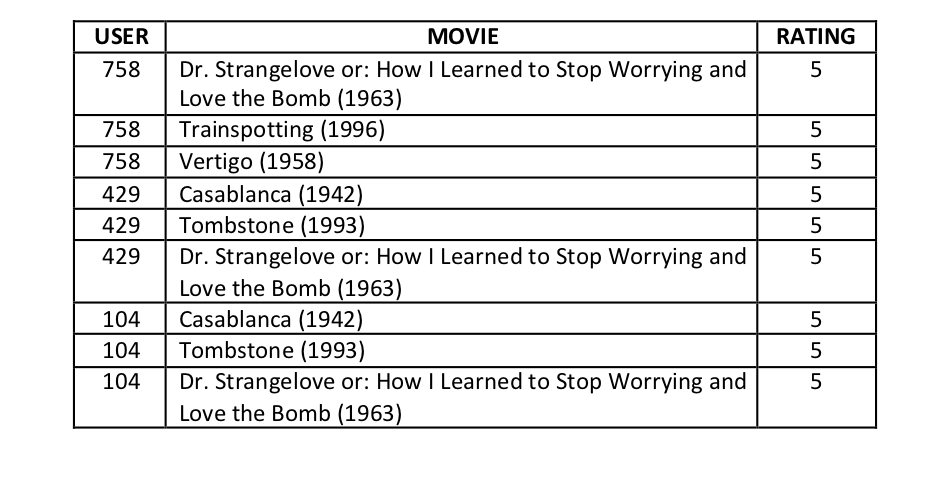
\includegraphics[width=0.6\textwidth]{top3}
     %\caption{Top 3 Favorite Movies}
	%\end{figure}

	
\end{homeworkProblem}
\clearpage
\newpage

%----------------------------------------------------------------------------------------
%   PROBLEM 2
%----------------------------------------------------------------------------------------

\begin{homeworkProblem}
2.  Using the PCI book modified docclass.py code and test.py (see Slack assignment-8 channel)\\
     Use your Training dataset to train the Naive Bayes classifier ( e.g., docclass.spamTrain() )\\
     Use your Testing dataset to test (test.py) the Naive Bayes classifier and report the classification results.\\
     
%\problemAnswer{

 \textbf{SOLUTION}\\
  		     
The below code files from text \textbf{Programming Collective Intelligence} 
has been modified to train and test the dataset.
		      
\begin{lstlisting}[language=Python, caption=docclass.py]
#from pysqlite2 import dbapi2 as sqlite
import sqlite3 as sqlite
import re
import math

def getwords(doc):
  splitter=re.compile('\\W*')
  #print(doc)
  # Split the words by non-alpha characters
  words=[s.lower() for s in splitter.split(doc) 
          if len(s)>2 and len(s)<20]
  
  # Return the unique set of words only
  toreturn = dict([(w,1) for w in words])
  return toreturn

class classifier:
  def __init__(self,getfeatures,filename=None):
    # Counts of feature/category combinations
    self.fc={}
    # Counts of documents in each category
    self.cc={}
    self.getfeatures=getfeatures
    
  def setdb(self,dbfile):
    self.con=sqlite.connect(dbfile)    
    self.con.execute('create table if not exists fc(feature,category,count)')
    self.con.execute('create table if not exists cc(category,count)')


  def incf(self,f,cat):
    count=self.fcount(f,cat)
    if count==0:
      self.con.execute("insert into fc values ('%s','%s',1)" 
                       % (f,cat))
    else:
      self.con.execute(
        "update fc set count=%d where feature='%s' and category='%s'" 
        % (count+1,f,cat)) 
  
  def fcount(self,f,cat):
    res=self.con.execute(
      'select count from fc where feature="%s" and category="%s"'
      %(f,cat)).fetchone()
    if res==None: return 0
    else: return float(res[0])

  def incc(self,cat):
    count=self.catcount(cat)
    if count==0:
      self.con.execute("insert into cc values ('%s',1)" % (cat))
    else:
      self.con.execute("update cc set count=%d where category='%s'" 
                       % (count+1,cat))    

  def catcount(self,cat):
    res=self.con.execute('select count from cc where category="%s"'
                         %(cat)).fetchone()
    if res==None: return 0
    else: return float(res[0])

  def categories(self):
    cur=self.con.execute('select category from cc');
    return [d[0] for d in cur]

  def totalcount(self):
    res=self.con.execute('select sum(count) from cc').fetchone();
    if res==None: return 0
    return res[0]


  def train(self,item,cat):
    features=self.getfeatures(item)
    # Increment the count for every feature with this category
    for f in features:
      self.incf(f,cat)

    # Increment the count for this category
    self.incc(cat)
    self.con.commit()

  def fprob(self,f,cat):
    if self.catcount(cat)==0: return 0

    # The total number of times this feature appeared in this 
    # category divided by the total number of items in this category
    return self.fcount(f,cat)/self.catcount(cat)

  def weightedprob(self,f,cat,prf,weight=1.0,ap=0.5):
    # Calculate current probability
    basicprob=prf(f,cat)

    # Count the number of times this feature has appeared in
    # all categories
    totals=sum([self.fcount(f,c) for c in self.categories()])

    # Calculate the weighted average
    bp=((weight*ap)+(totals*basicprob))/(weight+totals)
    return bp




class naivebayes(classifier):
  
  def __init__(self,getfeatures):
    classifier.__init__(self,getfeatures)
    self.thresholds={}
  
  def docprob(self,item,cat):
    features=self.getfeatures(item)   

    # Multiply the probabilities of all the features together
    p=1
    for f in features: p*=self.weightedprob(f,cat,self.fprob)
    return p

  def prob(self,item,cat):
    catprob=self.catcount(cat)/self.totalcount()
    docprob=self.docprob(item,cat)
    return docprob*catprob
  
  def setthreshold(self,cat,t):
    self.thresholds[cat]=t
    
  def getthreshold(self,cat):
    if cat not in self.thresholds: return 1.0
    return self.thresholds[cat]
  
  def classify(self,item,default=None):
    probs={}
    # Find the category with the highest probability
    max=0.0
    for cat in self.categories():
      probs[cat]=self.prob(item,cat)
      if probs[cat]>max: 
        max=probs[cat]
        best=cat

    # Make sure the probability exceeds threshold*next best
    for cat in probs:
      if cat==best: continue
      if probs[cat]*self.getthreshold(best)>probs[best]: return default
    return best

class fisherclassifier(classifier):
  def cprob(self,f,cat):
    # The frequency of this feature in this category    
    clf=self.fprob(f,cat)
    if clf==0: return 0

    # The frequency of this feature in all the categories
    freqsum=sum([self.fprob(f,c) for c in self.categories()])

    # The probability is the frequency in this category divided by
    # the overall frequency
    p=clf/(freqsum)
    
    return p
  def fisherprob(self,item,cat):
    # Multiply all the probabilities together
    p=1
    features=self.getfeatures(item)
    for f in features:
      p*=(self.weightedprob(f,cat,self.cprob))

    # Take the natural log and multiply by -2
    fscore=-2*math.log(p)

    # Use the inverse chi2 function to get a probability
    return self.invchi2(fscore,len(features)*2)
  def invchi2(self,chi, df):
    m = chi / 2.0
    sum = term = math.exp(-m)
    for i in range(1, df//2):
        term *= m / i
        sum += term
    return min(sum, 1.0)
  def __init__(self,getfeatures):
    classifier.__init__(self,getfeatures)
    self.minimums={}

  def setminimum(self,cat,min):
    self.minimums[cat]=min
  
  def getminimum(self,cat):
    if cat not in self.minimums: return 0
    return self.minimums[cat]
  def classify(self,item,default=None):
    # Loop through looking for the best result
    best=default
    max=0.0
    for c in self.categories():
      p=self.fisherprob(item,c)
      # Make sure it exceeds its minimum
      if p>self.getminimum(c) and p>max:
        best=c
        max=p
    return best


def sampletrain(cl):
  cl.train('Nobody owns the water.','good')
  cl.train('the quick rabbit jumps fences','good')
  cl.train('buy pharmaceuticals now','bad')
  cl.train('make quick money at the online casino','bad')
  cl.train('the quick brown fox jumps','good')

def spamTrain(cl):
  cl.train('the the', 'not spam')
  cl.train('cheap cheap cheap banking the', 'spam')
  cl.train('the', 'not spam')
  cl.train('cheap cheap banking banking banking the the', 'spam')
  cl.train('cheap cheap cheap cheap cheap buy buy the', 'spam')
  cl.train('banking the', 'not spam')
  cl.train('buy banking the', 'not spam')
  cl.train('the', 'not spam')
  cl.train('the', 'not spam')
  cl.train('cheap buy dinner the the', 'not spam')

def testEmail(cl):

    # training for non-spam
    for i in range(1,11):
        filename = 'Training/notspam' + str(i) +'.txt'
        with open(filename, 'r') as nonspam:
            cl.train(nonspam.read(), 'not spam')
  
    # training for spam
    for i in range(1,11):
        filename = 'Training/spam' + str(i) +'.txt'
        with open(filename, 'r') as spam:
            cl.train(spam.read(), 'spam')


\end{lstlisting}

\begin{lstlisting}[language=Python, caption=test.py]
import docclass
from subprocess import check_output

import numpy as np



def compareSample(file, pred):

    with open(file, 'r') as filename:
        result = cl.classify(filename.read())
        if result == 'spam':
            pred.append(1)
        else:
            pred.append(0)   
        
def emailTest(cl):

    outcome = [] 
    standard = np.array([1,1,1,1,1,1,1,1,1,1,0,0,0,0,0,0,0,0,0,0])
            
    # testing spam
    try: 
        for i in range(1, 11):
            filename = 'Testing/spam' + str(i) + '.txt'
            
            compareSample(filename, outcome)
                
    # testing non-spam
        for i in range(1, 11):
            filename = 'Testing/notspam' + str(i) + '.txt'
            compareSample(filename, outcome)
            
    except:
        print (filename)
        
    print ('STANDARD is:')
    print(standard)    
    outcome = np.array(outcome)

    print ('OUTCOME  after Comparison is:')
    print(outcome)
   
    truePositive = len(np.where(outcome[np.where(standard == 1)] == 1)[0])
    trueNegative = len(np.where(outcome[np.where(standard == 0)] == 0)[0])
    falsePositive = len(np.where(standard == 1)[0]) - truePositive
    falseNegative = len(np.where(standard == 1)[0]) - trueNegative
   
    confusionMatrix = [[truePositive, falsePositive], [falseNegative, trueNegative]]
    print('CONFUSION MATRIX is :')
    print (confusionMatrix)

    precision = float(truePositive) / (truePositive + trueNegative)
    accuracy = float(truePositive + falsePositive)/(truePositive + trueNegative + 
    falsePositive + falseNegative)
    print('PRECISION',float(precision))
    print('ACCURACY',float(accuracy))

    
cl = docclass.naivebayes(docclass.getwords)
check_output(['rm', 'spamCheck.db'])
cl.setdb('spamCheck.db')
docclass.testEmail(cl)
emailTest(cl)
\end{lstlisting}
%}

 
\end{homeworkProblem}
\clearpage
\newpage

%----------------------------------------------------------------------------------------
%   PROBLEM 3
%----------------------------------------------------------------------------------------

\begin{homeworkProblem}
3.  Draw a confusion matrix for your classification results\\
(see: https://en.wikipedia.org/wiki/Confusion_matrix)\\
%\problemAnswer{

 \textbf{SOLUTION}\\
 
With above generated dataset and the below formulae, i have arrived at the below confusion matrix.
Where 7 out of 10 spam email messages were predicted incorrectly as non-spam and only 3 of them were
predicted as spam.

\begin{figure}[h]
  \centering
    
\includegraphics[width=0.6\textwidth]{cmatrix}
     \caption{Confusion Matrix}
	\end{figure}
%}
\newpage
 
\end{homeworkProblem}

%----------------------------------------------------------------------------------------
%   PROBLEM 4
%----------------------------------------------------------------------------------------

\begin{homeworkProblem}
4.  Report the precision and accuracy scores of your classification results\\
(see: https://en.wikipedia.org/wiki/Precision_and_recall)\\

%\problemAnswer{

 \textbf{SOLUTION}\\
	
%}

To calculate the Precision and Accuracy for my dataset, i have made use of the below formulae from the suggested wikipedia page.

\begin{figure}[h]
  \centering
    
\includegraphics[width=0.6\textwidth]{precision}
     \caption{Precision Formula}
	\end{figure}
	
	Applying the parameters from the previous computation,i have arrived at below Precision
	\begin{verbatim}
	Precision = 0.3
	\end{verbatim}
	
\begin{figure}[h]
  \centering
    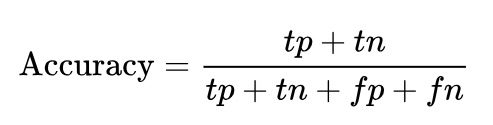
\includegraphics[width=0.6\textwidth]{accuracy}
     \caption{Accuracy Formula}
	\end{figure}
	
	Applying the parameters from the previous computation,i have arrived at below Accuracy
	\begin{verbatim}
	Accuracy = 0.5
	\end{verbatim}
	
\newpage
	
	
\end{homeworkProblem}

\textbf{References}
\begin{enumerate}
\item\textbf{} https://en.wikipedia.org/wiki/Confusion_matrix
\item\textbf{} https://en.wikipedia.org/wiki/Precision_and_recall)
\end{enumerate}
\end{document}
